% 
% Annual Cognitive Science Conference
% Sample LaTeX Paper -- Proceedings Format
% 

% Original : Ashwin Ram (ashwin@cc.gatech.edu)       04/01/1994
% Modified : Johanna Moore (jmoore@cs.pitt.edu)      03/17/1995
% Modified : David Noelle (noelle@ucsd.edu)          03/15/1996
% Modified : Pat Langley (langley@cs.stanford.edu)   01/26/1997
% Latex2e corrections by Ramin Charles Nakisa        01/28/1997 
% Modified : Tina Eliassi-Rad (eliassi@cs.wisc.edu)  01/31/1998
% Modified : Trisha Yannuzzi (trisha@ircs.upenn.edu) 12/28/1999 (in process)
% Modified : Mary Ellen Foster (M.E.Foster@ed.ac.uk) 12/11/2000
% Modified : Ken Forbus                              01/23/2004
% Modified : Eli M. Silk (esilk@pitt.edu)            05/24/2005
% Modified : Niels Taatgen (taatgen@cmu.edu)         10/24/2006
% Modified : David Noelle (dnoelle@ucmerced.edu)     11/19/2014

%% Change "letterpaper" in the following line to "a4paper" if you must.

\documentclass[10pt,letterpaper]{article}

\usepackage{cogsci}
\usepackage{pslatex}
\usepackage{apacite}
\usepackage{url}
\usepackage{graphicx}
\usepackage{caption}
\usepackage{subcaption}
\usepackage{listings}

\usepackage{amsmath}
\usepackage{amssymb}
\usepackage{wrapfig}


\newcommand*\diff{\mathop{}\!\mathrm{d}}
\newcommand{\denote}[1]{\mbox{ $[\![ #1 ]\!]$}}
\newcommand{\tableref}[1]{Table \ref{#1}}
\newcommand{\figref}[1]{Figure \ref{#1}}
\newcommand{\appref}[1]{Appendix \ref{#1}}
\newcommand{\sectionref}[1]{Section \ref{#1}}


\graphicspath{{img/}}

\title{``Not unreasonable'': The pragmatic logic of negated antonyms}
 
\author{{\large \bf Michael Henry Tessler (mhtessler@stanford.edu)} \\
  Department of Psychology, Stanford University 
  \AND {\large \bf Michael Franke (mchfranke@gmail.com)} \\
  Department of Linguistics, University of T\"{u}bingen}


\begin{document}

\maketitle


\begin{abstract}

If ``John is not unhappy'', does that mean that he's happy? 
The rules of logic make clear that two negations cancel each other out, but the same logic does not seem to hold in language. 
Instead, antonyms and their negations appear to partition the underlying semantic scale in an ordering: ``unhappy'' $<$ ``not happy'' $<$ ``not unhappy'' $<$ ``happy'' \cite{Horn1989:Natural, Krifka2007:Negated-antonyms}. 
We show how this semantic ordering falls out of an information-theoretic model of adjective interpretation, without assuming that ``unhappy'' $<$ ``happy''.
We then empirically investigate the semantic ordering, finding that the ordering appears when participants are fully aware of the utterances a speaker could say for antonym pairs defined by morphological negation (``[un]happy''); the explicit presentation of alternatives is not necessary for the analogous ordering of antonym pairs of distinct lexical items (``tall'' / ``short''). 
These findings suggest a model of interpretation where listeners maintain uncertainty about the parsing of an utterance involving multiple negations.


\textbf{Keywords:} 
semantics; pragmatics; Rational Speech Act; Bayesian cognitive model; adjectives
\end{abstract}


\section{Introduction}

Every introductory logic student understands that two negations cancel each other out: A ``not ungreen'' field is green.
Yet in natural language, there exist multiple, distinct ways of conveying negation.  
The morphology of a word can be altered to convey the opposite: ``un-'' + ``happy'' $\rightarrow$ ``unhappy''.
In addition, a negation-inducing modifier can be employed: ``not happy''.
Contra logic, however, these two ways of employing negation \emph{do not} cancel each other out: someone ``not unhappy'' is not necessarily happy. 	
As \citeA{Jespersen1924} noted:
%
\begin{quote}
The two negatives do not exactly cancel one another...; the longer expression is always weaker: ``this is not unknown to me'' or ``I am not ignorant of this'' means \emph{I am to some extent aware of it}, etc.
\end{quote}
%



\section{Computational model}

Gradable adjectives (e.g., ``tall'', ``happy'') convey the value along a scale (e.g., \emph{height}, \emph{happiness}) for some referent $x$ is above or below some contextually-specified threshold: $\denote{tall} = \emph{height}(x) > \theta$; $\denote{short} = \emph{height}(x) < \theta$.
\citeA{Lassiter2013} provided a probabilistic pragmatics model that constrains the threshold $\theta$ relative to a context, formalized by a prior distribution over the value of the scalar degree $x$.  
%
\begin{align}
L_{1}(x, \theta \mid u) &\propto S_{1}(u \mid x, \theta) \cdot P_(x) \cdot P(\theta) \label{eq:L1} \\
S_{1}(u \mid x, \theta) &\propto \exp{(\alpha_1 \cdot \ln {L_{0}(x \mid u, \theta)})} \label{eq:S1}\\
L_{0}(x \mid u, \theta) &\propto {\delta_{[\![u]\!](x, \theta)} \cdot P_{c}(x)} \label{eq:L0}
\end{align}
%
This is a Rational Speech Act (RSA) model, a recursive Bayesian model where speaker $S$ and listener $L$ coordinate on an intended meaning \cite<for a review, see >{Goodman2016:RSA}.
In this framework, the pragmatic listener $L_1$ tries to resolve the state of the world $x$ (e.g., the height) from the utterance she heard $u$ (e.g., ``tall'').
She imagines the utterance came from an approximately rational Bayesian speaker $S_1$ trying to inform a naive listener $L_0$, who in turn updates her prior beliefs $P_(x)$ via an utterance's literal meaning $[\![u]\!](x)$.
$\theta$ comes from an uninformed prior and is resolved by the listener by reasoning about the likely states of the world $P_(x)$ (e.g., possible heights) and the likelihood that a speaker would say the adjective given a state and a threshold $S(u \mid x, \theta)$.


\section{Experiment 1: Measuring the ordering}
\subsection{Methods}
\subsubsection{Participants}

We recruited 120 participants from Amazon's Mechanical Turk (MTurk). 
This number was arrived it with the intention of getting approximately 25 ratings for each unique item in the experiment.
In all experiments, participants were restricted to those with U.S. IP addresses and who had at least a 95\% work approval rating. 
The experiment took on average N minutes and participants were compensated \$N for their work.

\subsubsection{Materials}

We used adjective quartets composed of positive-form gradable adjectives (\emph{POS}; e.g., ``happy''), their antonym (\emph{ANT}; e.g., ``unhappy''), and their respective negations (\emph{NEG POS}, ``not happy''; \emph{NEG ANT} ``not unhappy''); we refer to these four \emph{sentence types} collectively as an \emph{antonym quartet}.
Antonyms were either created by morphological negation (\emph{morphological antonyms}; e.g., ``unhappy'' for ``happy'') or were distinct lexical entries (\emph{lexical antonyms}; e.g., ``short'', for ``tall'').
All adjectives were individual-level predicates that applied to people; items were constructed from an informal survey of the linguistics literature and taken from list of ``common opposites'' available online\footnote{http://www.enchantedlearning.com/wordlist/opposites.shtml} (for a full list, see \tableref{tab:items}.

\begin{table}[b]
\centering
\begin{tabular}{l|l}
\emph{Morphological antonyms}     & \emph{Lexical antonyms}    \\ 
\hline
happy, unhappy             & tall, short         \\
intelligent, unintelligent & rich, poor          \\
polite, impolite           & fat, skinny         \\
interesting, uninteresting & hard-working, lazy  \\
attractive, unattractive   & brave, cowardly     \\
successful, unsuccessful   & beautiful, ugly     \\
honest, dishonest          & wise, foolish       \\
educated, uneducated       & proud, humble       \\
friendly, unfriendly       & strong, weak        \\
mature, immature           & loud, quiet        
\end{tabular}
\caption{Antonym pairs used in Experiments 1 \& 2}
\label{tab:items}
\end{table}


\subsubsection{Procedure}

On each trial, participants read a statement introducing a character using a gradable adjective in one of the four \emph{sentence types} (e.g., ``Greg is \{POS, ANT, NEG POS, NEG ANT\}'').
Participants were asked to interpret the statement by placing the character on a scale from ``the most POS person'' to ``the most NEG person'', using a slider bar (\figref{fig:expt1}).
Participants completed 16 trials; each used a different adjective quartet.
Throughout the course of the experiment, participants saw 2 of each \emph{sentence type} with both \emph{lexical} and \emph{morphological} antonym quartets. 

\begin{figure*}[t]
	\centering
	\begin{subfigure}[t]{0.5\textwidth}
		\centering
		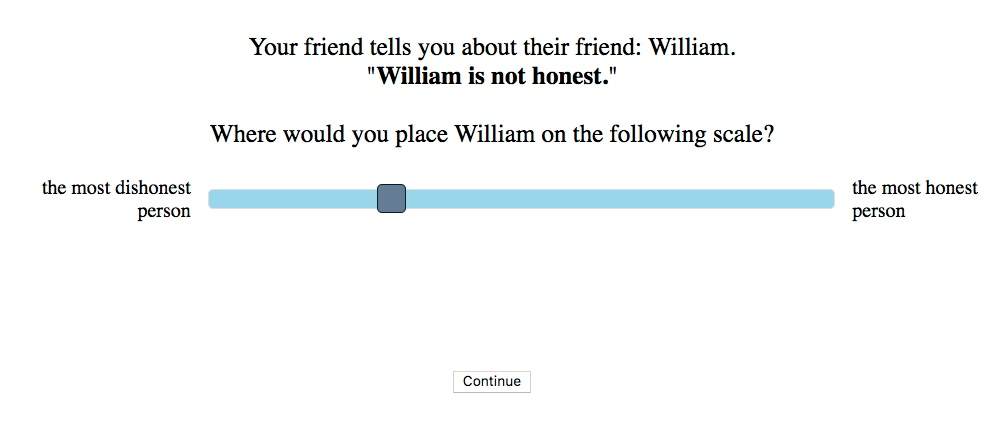
\includegraphics[width=\textwidth]{expt1.jpeg}
		\caption{Experiment 1}\label{fig:expt1}		
	\end{subfigure}%
	\begin{subfigure}[t]{0.5\textwidth}
		\centering
		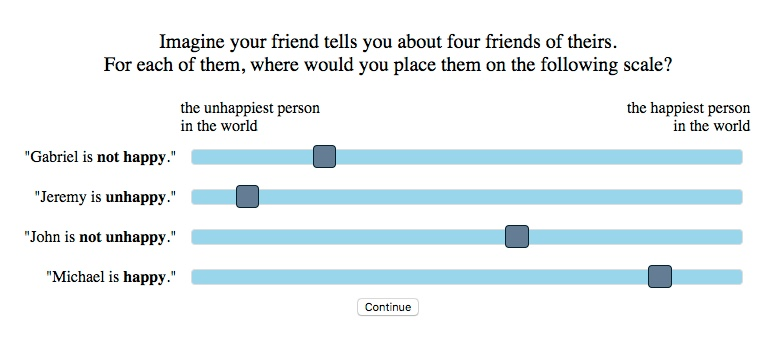
\includegraphics[width=\textwidth]{expt2.jpeg}
		\caption{Experiment 2}\label{fig:expt2}
	\end{subfigure}
	\caption{Example experimental trials.}\label{fig:expt-procedure}
\end{figure*}



\subsection{Results}

X participants were excluded for self-reporting a native language other than English. 


\section{Experiment 2: Explicit alternatives}
This experiment was designed in order to test the influence of salient alternatives on the hypothesized semantic ordering for antonym quartets.

\subsection{Methods}

\subsubsection{Participants}

We recruited 50 participants MTurk.
This number was arrived it with the intention of getting approximately 25 ratings for each unique item in the experiment.
The experiment took on average N minutes and participants were compensated \$N for their work.


\subsubsection{Materials and Procedure}
The experimental materials were the same as in Expt.~1. 
The procedure differed in that participants saw and rated all four sentence types simultaneously (\figref{fig:expt2}). 
In addition, the endpoints of the slider bars were relabeled to ``the most \{\emph{POS}, \emph{ANT}\} person \emph{in the world'}'; excluding the ``in the world'' phrase leads to a salient interpretation of the endpoints as indicating ``the most \emph{POS} person (of these four)''.

\subsection{Results}


\section{Acknowledgments}


\bibliographystyle{apacite}

\setlength{\bibleftmargin}{.125in}
\setlength{\bibindent}{-\bibleftmargin}

\bibliography{negant}


\end{document}
